\label{sec:vbf-uncertainties}

Several sources of systematic uncertainties,
affecting the normalization of signal and background and/or the shape of
the distributions used in this analysis, have been considered.  Individual sources of systematic 
uncertainty are considered uncorrelated. The systematic variations with less than $0.5\%$ impact 
on the yields in a particular BDT region will be ignored in the profile likelihood fit for 
that particular region. 

\subsubsection{Luminosity}
\label{sec:vbf-syst_lumi}

The integrated luminosity measurement has an uncertainty of 3.4\%. This systematic uncertainty
is applied to all physics processes estimated with MC simulated samples normalized 
to the measured integrated luminosity: \zjets{} and Higgs production.

\subsubsection{Uncertainties on object definitions}
\label{sec:vbf-syst_objects}

Several uncertainties are applied to the MC simulation samples to take into account the limited knowledge of the detector and reconstruction performance.

\paragraph{Trigger efficiencies}

The per-jet online \btagging efficiency with respect to the offline \btagging efficiency is measured in $t\bar t$ events. 
To cover the event topology dependence, a scale factor applied to the leading b-tagged jet is derived as a function of the jet $\eta$. 

\paragraph{JVT efficiency}
The per-jet efficiency to satisfy the jet vertex tagging requirement
is measured in $Z(\to \ell^+\ell^-)$+1-jet events in data and simulation,
selecting separately events enriched in hard-scatter jets and events enriched in pile-up jets. 
The corresponding uncertainty is evaluated by shifting the per-jet scale factors,
accounting for the efficiency uncertainty~\cite{JVTwiki}.

\paragraph{Jet energy scale}
%\label{sec:vbf-syst_jes}

The jet energy scale and its uncertainty have been derived combining information from test-beam data, 
LHC collision data and simulation \cite{JESwiki}. The jet
energy scale uncertainty is split into 4 uncorrelated sources, 
which can have different jet $\pt$ and $\eta$ dependencies.  These sources are
treated independently in this analysis, using the \texttt{JetUncertainties} tool \cite{TWiki_JetUncertainties} 
to compute the uncertainties corresponding to each eigenvector. 
The variation in the jet energies as a result of these systematic uncertainties are also propagated through all
observables computed using jet kinematics.

\paragraph{Jet energy resolution}
%\label{sec:vbf-syst_jer}
The jet energy resolution (JER) has been measured separately for data and simulation 
using in-situ techniques. The \texttt{JERUncertaintyProvider}
tool~\cite{jeruncertaintyprovider} was used to obtain the expected fractional
$p_T$ resolution for a given jet as a function of its $p_T$ and rapidity. 
The systematic uncertainty is taken by smearing the jet energy by the shift 
in resolution provided by the tool and comparing to the nominal
shape and normalization in simulation. 
The nominal value is used as the default in the analysis.

In order to propagate the uncertainty in the $p_T$ resolution, for each jet a 
random number $r$ is drawn from a Gaussian distribution with mean 0 and sigma equal 
 to the difference in quadrature between the fractional $p_T$ resolution with the tool and the nominal
one.  The jet 4-momentum is then scaled by a factor $1+r$.  By definition, such uncertainty
is one-sided, since jets in simulation cannot be made to have a better resolution than exists in the simulation.
We compute the normalization and shape uncertainties in the final distributions 
and symmetrize them to define a corresponding ``down'' variation.

\paragraph{\btagging}
%\label{sec:vbf-syst_btag}

Simulation efficiencies for $b$ and $c$ quarks have to be corrected by a
$\pt$-dependent factor. In the case of light flavor jets, the corrections also 
depend on jet $\eta$. 
Each uncertainty corresponds to a resulting eigenvector after diagonalizing the matrix
containing the information of total uncertainty per $\pt$ bin and the bin-to-bin 
corrections. These systematic
uncertainties are taken as uncorrelated between $b$, $c$, and light flavor jets.
A per-jet weighting procedure is applied to simulated events to propagate the 
calibration of $b$-tagging and the related uncertainties. 
The correlation across operating points is ignored. It has been checked that this choice
wouldn't impact the results by considering the uncertainties fully correlated or fully uncorrelated.


\paragraph{Track multiplicity for Quark/gluon separation}

The track multipicity discrimination power for quark/gluon separation in simulation 
is affected by the modeling of the charged multiplicity in jet fragmentation and the modeling of the
track multiplicity reconstruction. The estimation of the corresponding uncertainties is 
described in Ref.~\cite{qgtagging}. A total of 5 nuisance parameters is used to parametrize these
uncertainties and the impact on the results presented in this thesis is found to be negligible.

\paragraph{Non-resonant background}
The non-resonant background is modeled with an analytical function, either O(3) or O(4) Bernstein polynomial. 
The potential local bump or dip caused by the functional choice is characterized by spurious signal 
which is derived by fitting the nominal model plus signal to an alternative model. The derived spurious signal 
size is then quoted the width of a gaussian constraint which is included in the profile likelihood as in 
Eq.~\ref{likelihood}.

%\paragraph{\zjets{} normalization}
%\label{sec:vbf-zjets}
%
%Strategy~\label{item:z-treat-5} of section~\ref{sec:vbf-ztreat} is taken for the systematic uncertainties on the \zjets{} normalization.
%
%The bias on the signal $\mu$ value caused by this rescaling (or lack thereof) is estimated 
%with an injection test where the scaled pseudodata is fit with the non-scaled template. 
%The bias is found to be less than $10\%$ and therefore negligible with respect to the overall uncertainty.
%Therefore no relative rescaling is applied to the \zjets{} MC prediction in each region.
%Additional details of these studies are provided in Appendix ~\ref{sec:vbf-app-zmm}.

%The normalization of the \zjets{} background, simulated at LO, is 
%affected by potentially large uncertainties~\cite{zkfactors}. 
%In order to estimate the \zjets{} normalization in data, the $Z(\mu\mu)+$jets yield
%is used as proxy. The ratio between data and MC yield after preselection is used to estimate the overall
%normalization and the difference between \zjets{} and $Z(\mu\mu)+$jets is 
%taken as uncertainty.
%The data/MC ratio is found to be 0.74(0.1) and 0.79(0.1) for \twocentral and \fourcentral channels respectively. 
%A single gaussian NP with width 0.1 is therefore used in the global fit. 
%The $Z(\mu\mu)+$jets sample is also used to study the variation across signal and control regions.
%The \zjets{} prediction is scaled in each BDT region by the ratios between the yields observed in $Z(\mu\mu)+$jets data
%and in \zjets{} and $Z(\mu\mu)+$jets MC. The scale factors are listed in Table~\ref{tab:z_ratios}
% 

\paragraph{QCD Scale Variations}

The QCD scale uncertainty for VBF is taken as varying the renormalization
and factorization scales together by a factor of 2 and 0.5. As indicated in ~\cite{QCDscale_vbf}, 
this treatment in general leads to larger variations than the independent variation of renormalization
and factorization scales. 

The QCD scale uncertainty for ggF follows the \textit{2017 scheme} recommended by 
LCH Higgs working group, which is a group to produce agreements on Higgs theoretical properties,
in the follow-up of March meeting 2017 ~\cite{QCDscale_ggF}. In total, nine independent 
variations in six categories are considered. The terms and corersponding uncertainty sources 
are the following:

\begin{enumerate}
\item \textit{mu}, factorization scale variation
\item \textit{res}, renormalization scale variation
\item \textit{vbf2j} and \textit{vbf3j}, VBF topology uncertainties
\item \textit{mig01} and \textit{mig12}, truth level bin migration for non-Higgs jets
\item \textit{pTH60} and \textit{pTH120}, uncertainties extrapolation with Higgs $p_T$
\item \textit{qmt}, uncertainties of top quark mass
\end{enumerate}

The dominant source of uncertainty for this analysis comes from the term \textit{mig12} (size of $~17-18\%$), 
which is the leading source of uncertainty in high $p_T(H)$ event topology. 

Naively, one would assume uncertainties due to VBF topology terms are considerable. 
However, it is worth noting that these terms only matter for events which 
at truth level are generated in VBF topology. An event falls into Stage one classification 
of VBF topology if the truth Higgs has $p_T<200GeV$ and 
\begin{enumerate}
\item $MJJ>400 GeV$ and $|\textnormal{y(J1)-y(J2)}|>2.8$ ( loose VBF, events having $>3$ jets),
\item Pass loose VBF selection $\overrightarrow{p_{T}}(J1)+\overrightarrow{p_{T}}(J2)+\overrightarrow{p_{T}}(Higgs)<25GeV$ (tight VBF, events having ~2 jets),
\end{enumerate}
where the VBF jets are defined as the leading two jets aside from the Higgs. We note that $80\%$ of the events have $p_T(H)>200GeV$ and 
these events would not fall into the VBF category. Hence, the VBF topology uncertainties would not even apply in the \textit{2017 scheme} for most of our events. 
For our application, we could extend the definition of VBF topology to high $p_T(H)$ events and take the \textit{vbf2j} and \textit{vbf3j} values
for low $p_T(H)$ VBF topology to be the uncertainty for high $p_T(H)$ events as well. (\textit{vbf2j} and \textit{vbf3j} are defined as constants.)

We also notice that the \textit{2017 scheme} has a different definition of VBF jets, which selects the leading two jets aside from Higgs,  from the 
offline selection we apply in this analysis, which seeks a pair of jets that maximizes the $MJJ$ value. Hence if an event which is categorized by \textit{2017 scheme}
as non-VBF, the scheme lacks a term to properly count the 2J VS. 3J truth event topology uncertainty. Therefore, we also propagate the VBF topology 2J VS. 3J
uncertainties to standard non-VBF ggF+GE2j category. 

Overall, if VBF topology uncertainties are only applied to low $p_T(H)$ events, this source 
of ucnertainty is $<3\%$ in all signal regions. If the uncertainty is extended to high $p_T(H)$ events and as well as non-VBF ggF+GE2j events, the uncertainty
is about $20\%$. We take this very conservative extended version of uncertainty for ggF events.

%\begin{table}[htbp]
%\centering
%\caption{Fraction of ggF events in high $p_T(H)$ and VBF topology category}
%\label{tab:highpTfraction}
%\begin{tabular}{|l|l|l|l|l|l|l|}
%Region   & 2cen SR I & 2cen SR II & 4cen SR I & 4cen SR II & 4cen SR III & 4cen SR IV \\
%Fraction & 17.5\%    & 10.4\%     & 13.2\%    & 19.4\%     & 8.8\%       & 9.5\%     
%\end{tabular}
%\end{table}


\paragraph{PDF}
The uncertainty on the PDF description used to simulate the signal is evaluated
by varying the PDF based on the uncertainties along each of the PDF eigenvectors.
Each variation is applied by reweighting the signal samples event-by-event.
A single nuisance parameter, corresponding to the envelope of all the variations,
is considered.

\paragraph{Parton Shower}

The modeling of parton shower could directly affect observables which are heavily 
correlated with the jettiness of the event. In this analysis, its impact is most 
prominent on $p_{T}$ balance, which is a variable used as the BDT input. The nominal
Pythia sample is compared with the \herwig{} sample at the truth level to derive a 
reweighting map for $p_{T}$ balance.
This reweighting map is then applied to the observable of the reconstructed events. The full impact of this variation 
is evaluated by running the BDT analysis while fixing other variables at their nominal 
and applying reweighting of $p_{T}$ balance. 


\paragraph{Signal Contamination from \VH and \ttH Processes}

The cross section of other Higgs production mode like \VH and \ttH are comparable to
the VBF process. Events from \VH (fully hadronic final states) and \ttH production could 
also pass the event selections of this analysis. The \Mbb distributions of these process
 are shown in Figure~\ref{fig:Mbb-ttH-VH}. The yields of these processes are presented 
in Table~\ref{tab:vh-tth-yield}.  The contributions to the total Higgs yields are  small 
in the most sensitive signal regions (0.2 -- 0.8 \%),  and rise to 15\% in the least sensitive regions.  

The VH process has a prominent resonance peak, similar to the VBF and ggF distributions. However, 
the statistics of the Monte Carlo sample is low, especially in \twocentral channel. 
We assign a 100\% uncertainty to the \VH process yield for a conservative estimate of 
the \VH contribution. %Its yield is added to the Higgs yields from VBF and ggF processes.

The \ttH mass distribution is a combination of the resonance peak and a continuum. 
The continuum arises from the fact that the \ttH process has at least four $b$-jets in the final state.
The failure of the jet assignment to identify the correct Higgs daughter $b$-jets results in a 
continuum combinatorial background which can be clearly seen in Figure~\ref{fig:Mbb-ttH-VH}. 
The yield is also assigned with 100\% uncertainty.
%In the fit, we take the actual shape of \ttH treating it as a background. 


\begin{figure}[htbp]
  \centering
 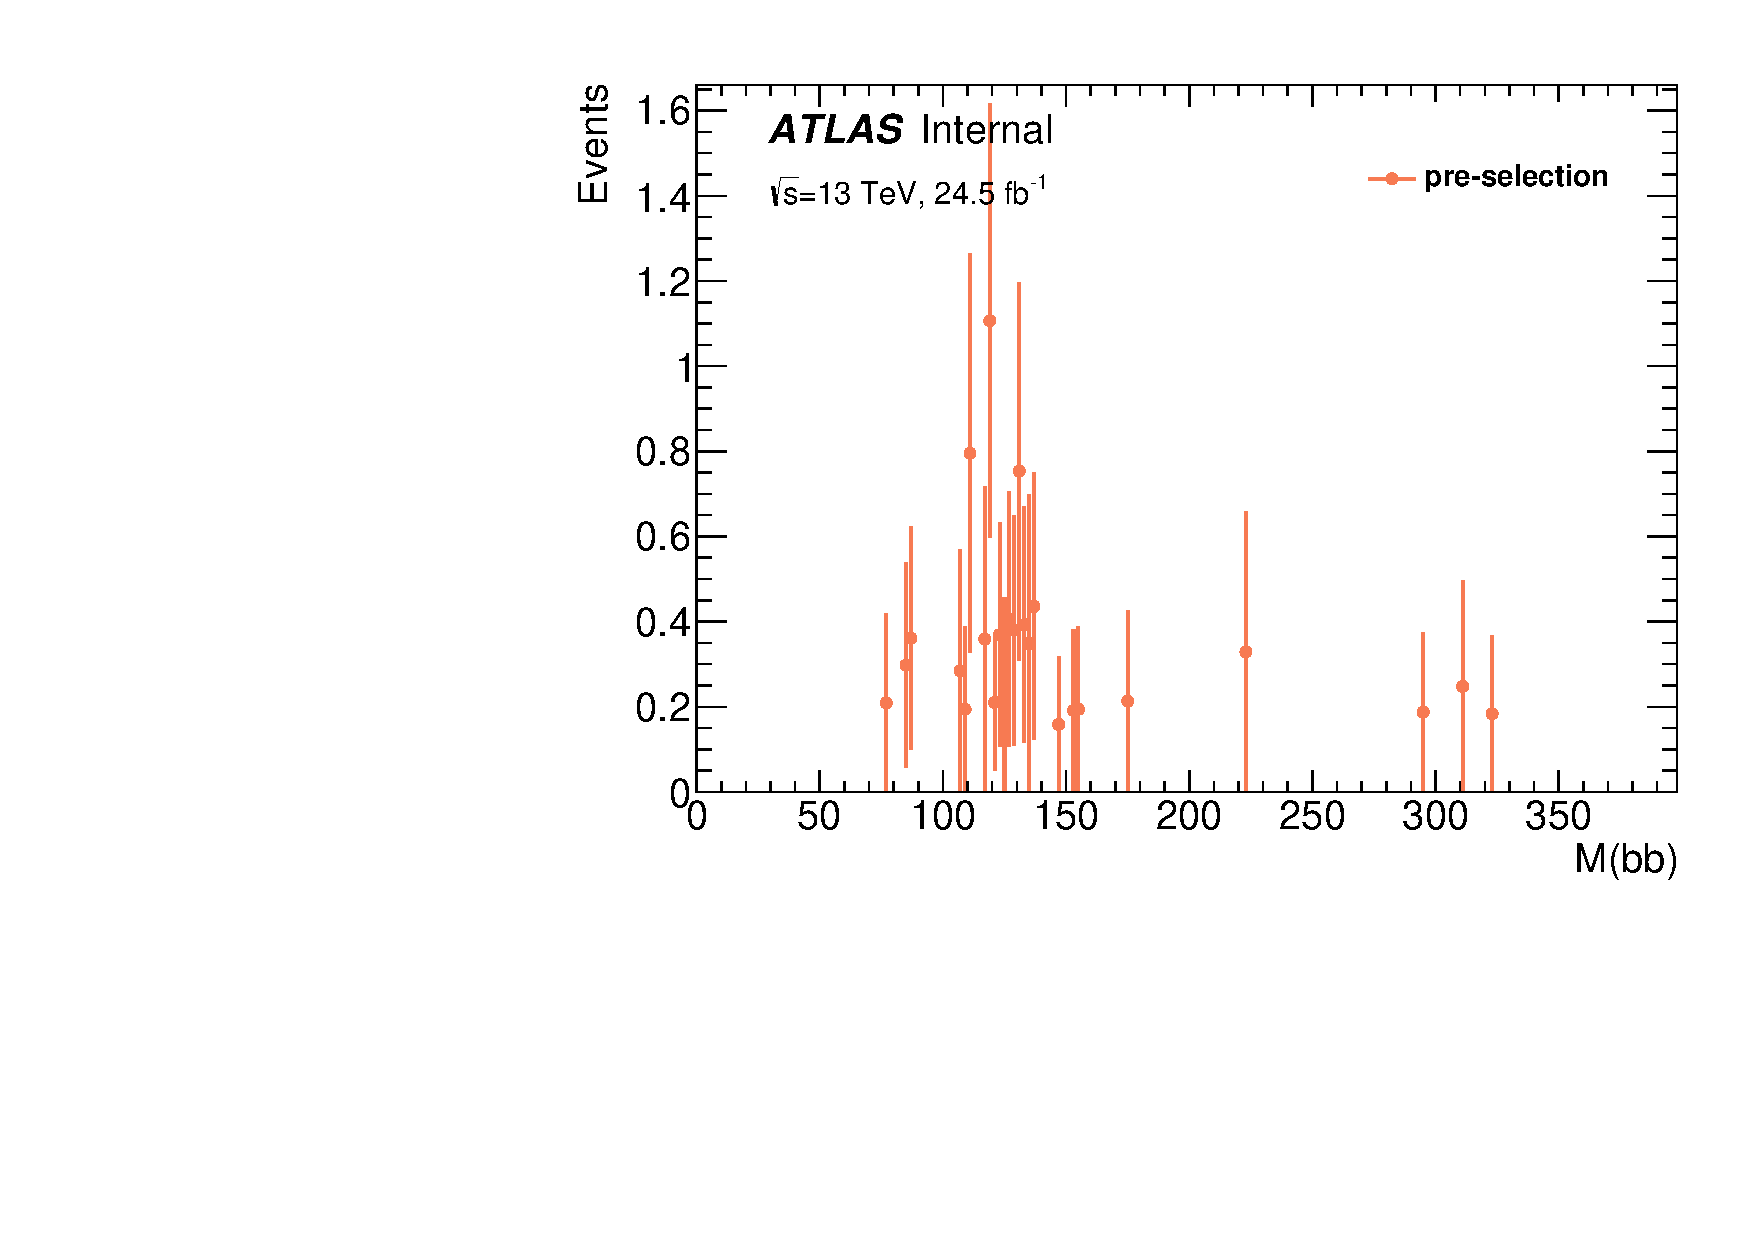
\includegraphics[width=0.35\textwidth]{figures/VBF/Mbb_VH_2cen.pdf}
 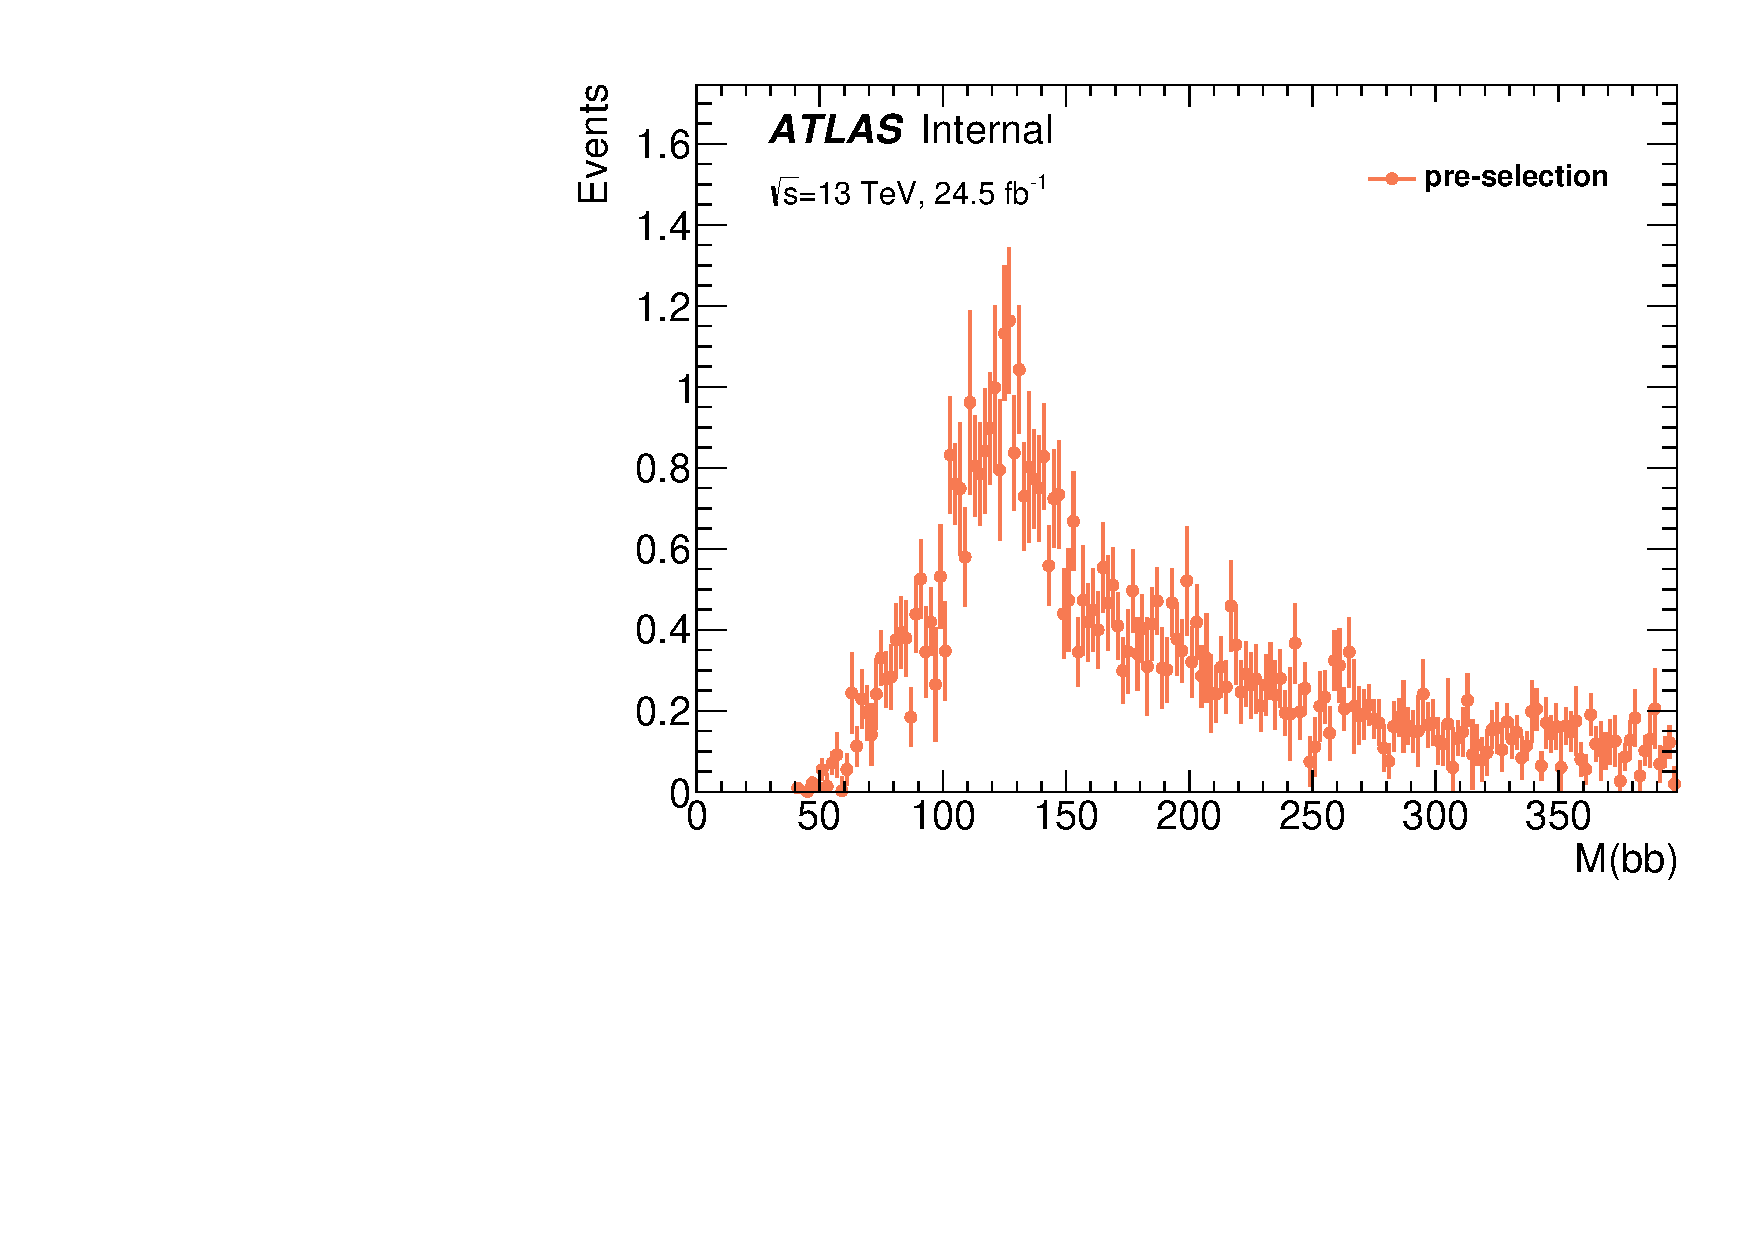
\includegraphics[width=0.35\textwidth]{figures/VBF/Mbb_ttH_2cen.pdf}\\
 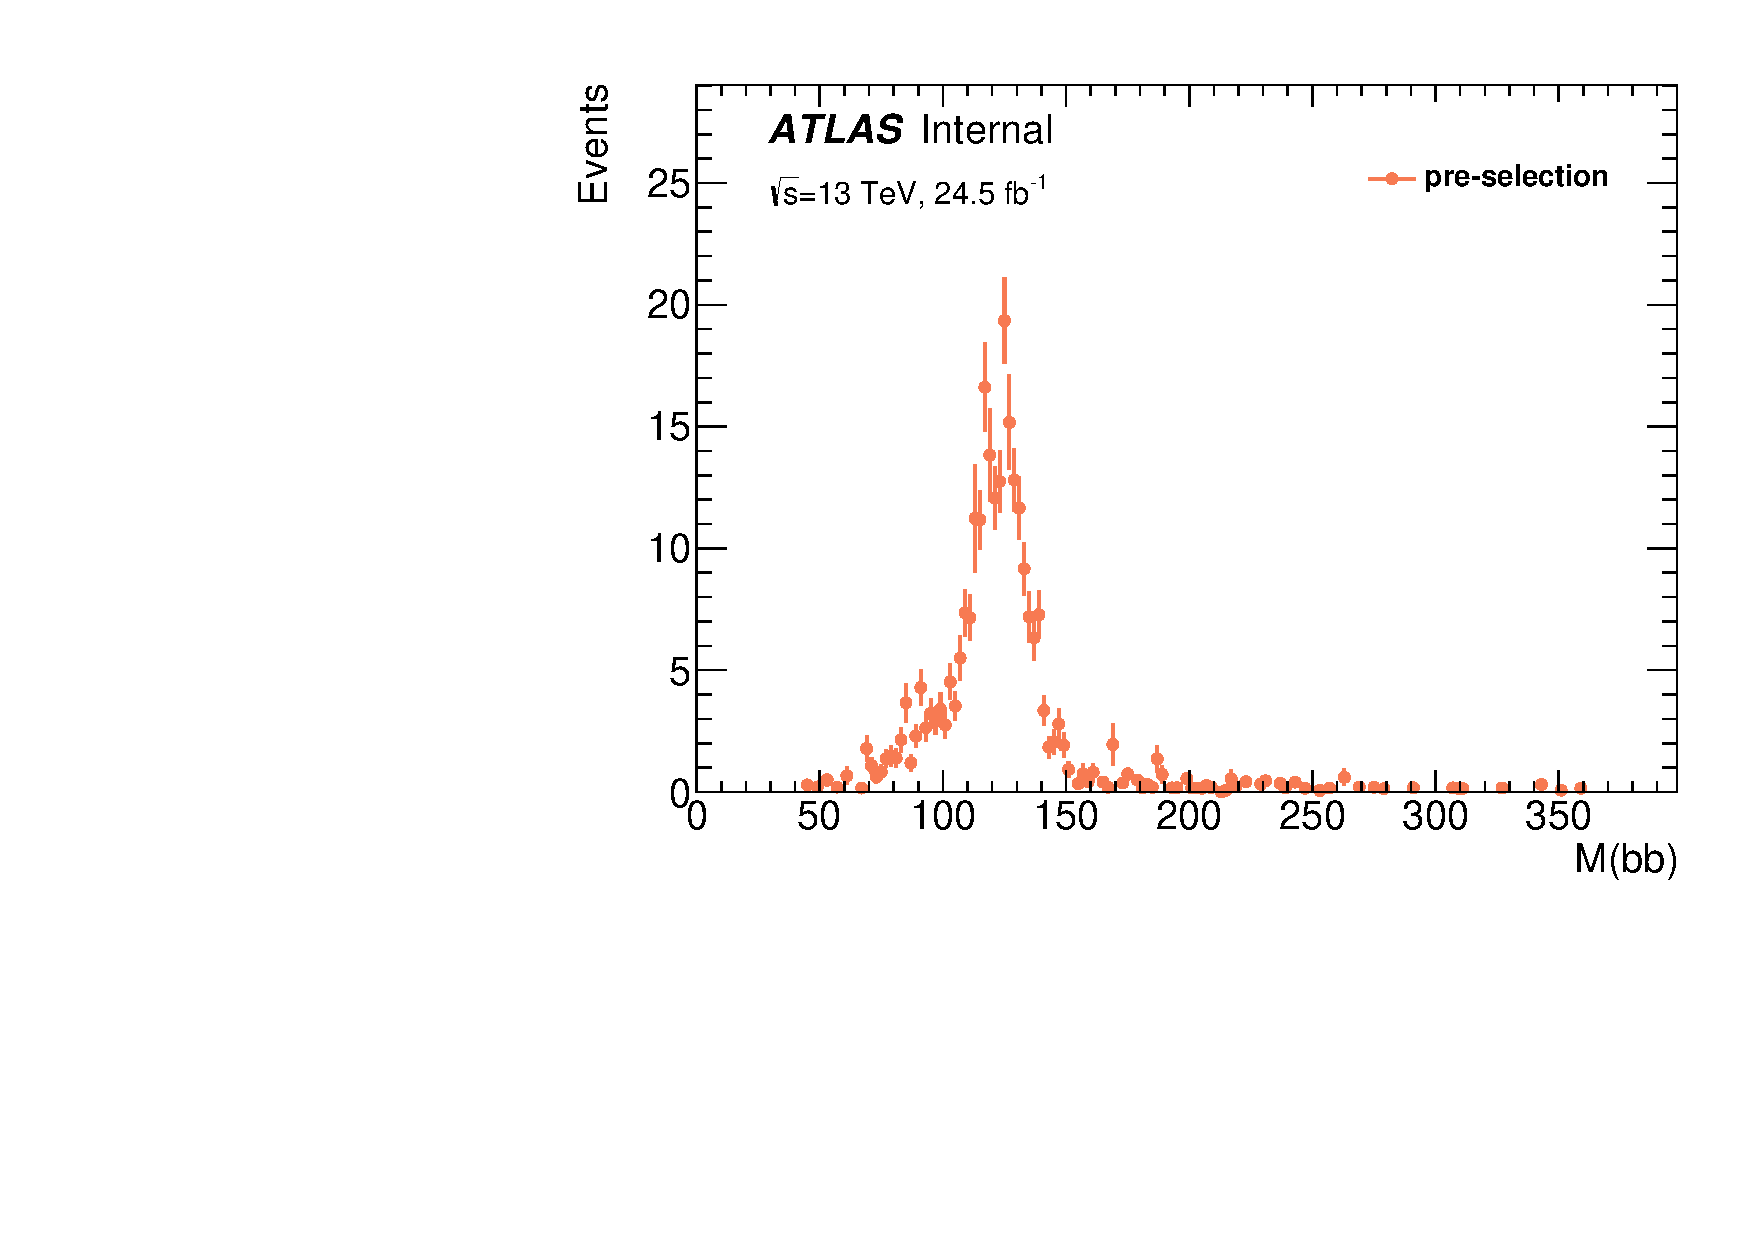
\includegraphics[width=0.35\textwidth]{figures/VBF/Mbb_VH_4cen.pdf}
 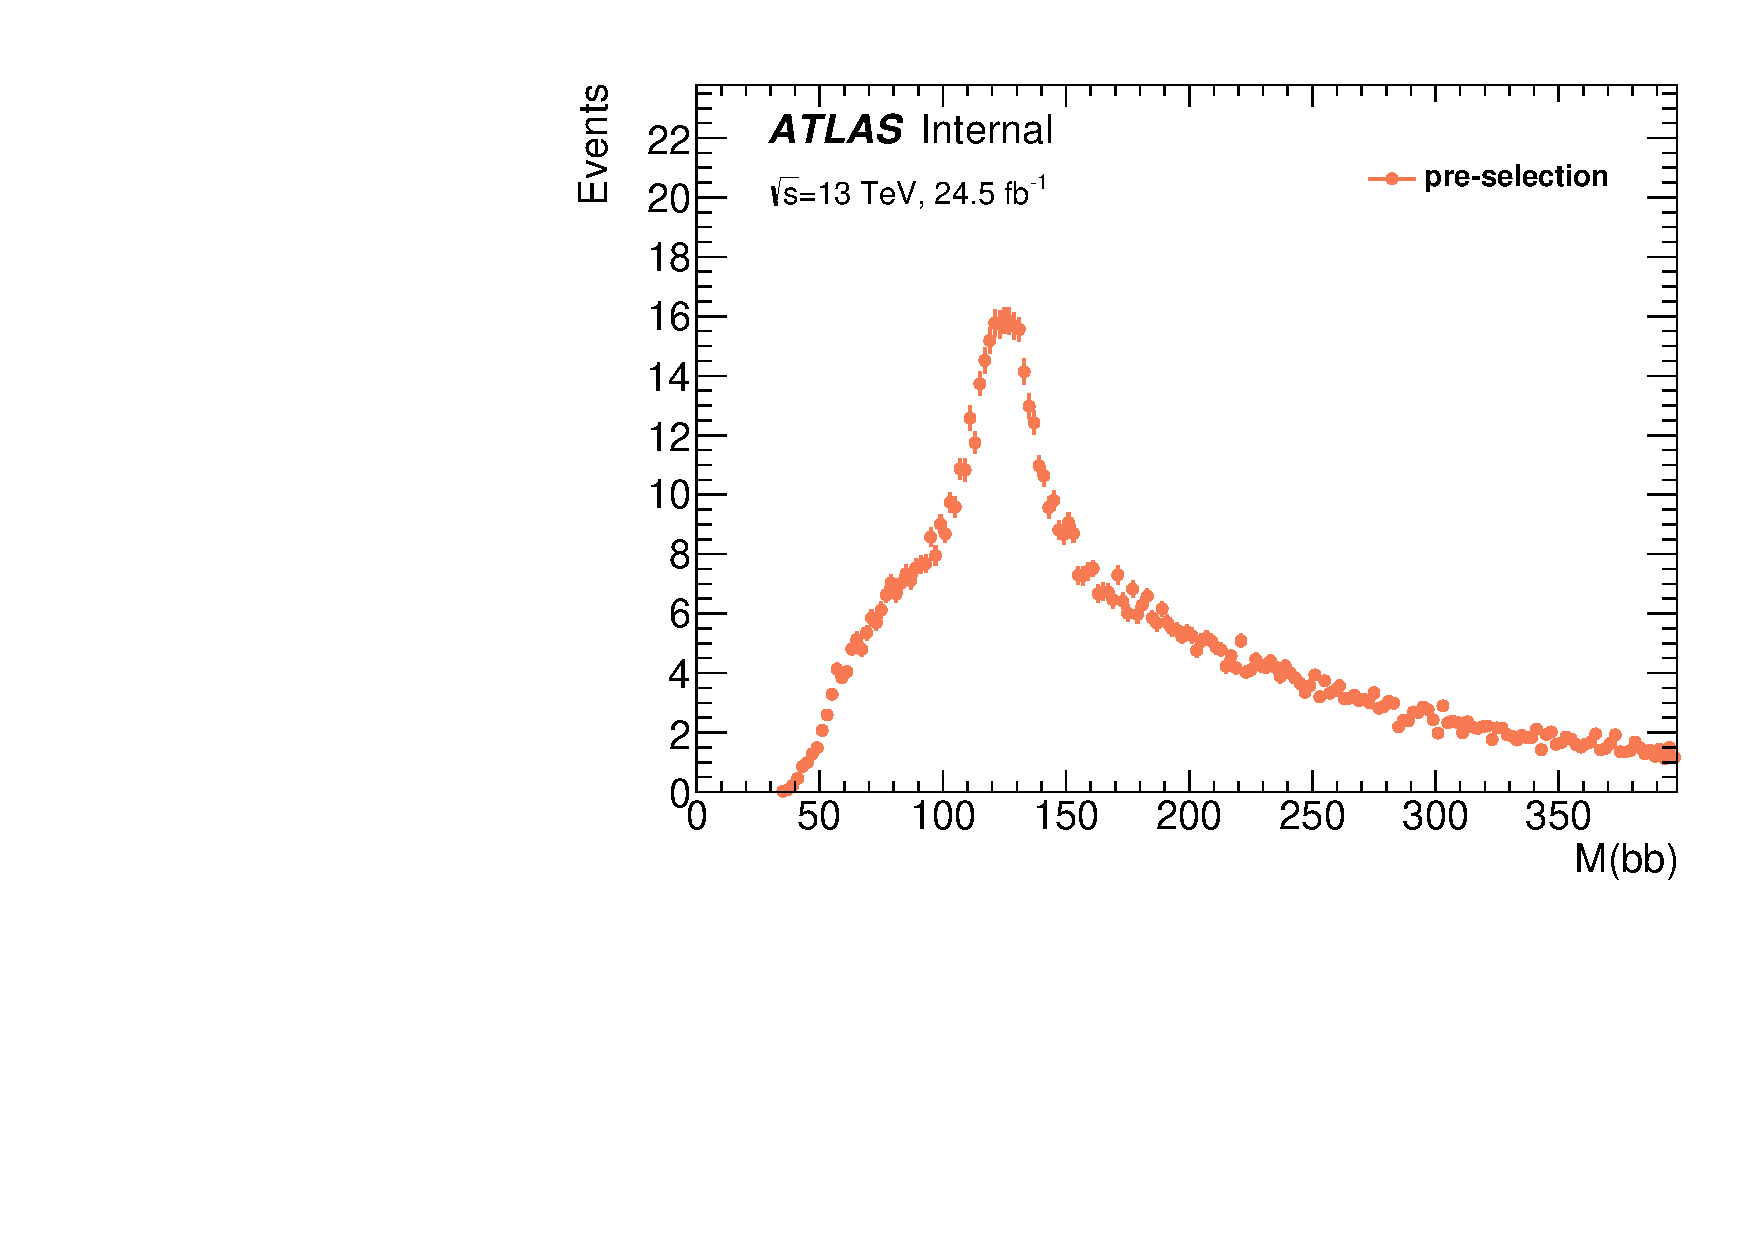
\includegraphics[width=0.35\textwidth]{figures/VBF/Mbb_ttH_4cen.pdf}
 \caption{\Mbb distributions of \VH (left) and \ttH (right) for \twocentral (top) and \fourcentral (bottom) channels passing event pre-selection. }
  \label{fig:Mbb-ttH-VH}
\end{figure}

\begin{table}[htbp]
\centering
\caption{Yields of \VH and \ttH}
\label{tab:vh-tth-yield}
\begin{tabular}{|l|l|l|l|l|}
\hline
     & \multicolumn{2}{l|}{\twocentral SR I}    & \multicolumn{2}{l|}{\twocentral SR II}  \\ \hline
     & Expected Yied  & Fraction of Total Yield & Expected Yied & Fraction of Total Yield \\ \hline
\VH  & 0.2           & 0.2\%                  & 9.3          & 6.8\%                  \\ \hline
\ttH & 4.2           & 2.9\%                  & 30.0         & 19.7\%                 \\ \hline
     & \multicolumn{2}{l|}{\fourcentral SR I}   & \multicolumn{2}{l|}{\fourcentral SR II} \\ \hline
     & Expected Yied  & Fraction of Total Yield & Expected Yied & Fraction of Total Yield \\ \hline
\VH  & 1.4           & 2.0\%                  & 0.7          & 1.4\%                  \\ \hline
\ttH & 0.6           & 0.8\%                  & 2.2          & 4.2\%                  \\ \hline
     & \multicolumn{2}{l|}{\fourcentral SR III} & \multicolumn{2}{l|}{\fourcentral SR IV} \\ \hline
     & Expected Yied  & Fraction of Total Yield & Expected Yied & Fraction of Total Yield \\ \hline
\VH  & 6.0           & 5.2\%                  & 34.1         & 13.5\%                  \\ \hline
\ttH & 12.4          & 10.2\%                 & 42.4         & 15.5\%                 \\ \hline
\end{tabular}
\end{table}

\clearpage

\subsubsection{Summary}
The typical signal yield changes due to a few representative systematic uncertainties are 
shown in Tables. \ref{tab:syst-2cen} and \ref{tab:syst-4cen}.  The theory uncertainties, especially from the QCD scale dominate, at the 20\% level across all signal regions.  The largest experimental uncertainties are from \btagging, at the 3--4\% level.

\begin{table}[hbpt]
\centering
\scriptsize
\begin{tabular}{|l|l|l|l|l|l|l|}
\hline
                 & \multicolumn{6}{c|}{\twocentral}                     \\ \hline
                 & \multicolumn{3}{c|}{SRI} & \multicolumn{3}{c|}{SRII} \\ \hline
                 & Total  & VBF    & ggF    & Total   & VBF    & ggF    \\ \hline
Jet Energy Scale NP1           & 0.75   & 1.19   & 1.14   & 2.54    & 4.11   & 2.07   \\ \hline
Jet Energy Scale \bjets        & 1.52   & 1.62   & 1.08   & 2.21    & 2.71   & 2.06   \\ \hline
Jet Energy Resolution          & 1.65   & 3.03   & 4.11   & 2.16    & 4.69   & 4.19   \\ \hline
\qgtagging                     & 0.65   & 0.73   & 0.28   & 1.39    & 2.12   & 1.18   \\ \hline
Pile-up Reweighting            & 0.49   & 0.18   & 1.74   & 0.18    & 0.99   & 0.54   \\ \hline
\btagging NP0 70WP             & 2.66   & 2.67   & 2.60   & 2.88    & 2.74   & 2.92   \\ \hline
\btagging NP0 85WP             & 0.80   & 0.87   & 0.52   & 1.26    & 1.08   & 1.31   \\ \hline
$\alpha_s$                     & 0.73   & 0.14   & 3.18   & 2.66    & 3.95   & 3.35   \\ \hline
QCD scale VBF                  & 9.92   & 12.29  & 0      & 2.41    & 10.50  & 0      \\ \hline
QCD scale ggF                  & 8.17   & 0      & 42.33  & 29.61   & 0      & 41.91  \\ \hline
PDF Variations                 & 10.08  & 11.52  & 4.16   & 6.36    & 9.56   & 5.42   \\ \hline
Parton Shower                  & 0.34   & 1.06   & 2.69   & 0.62    & 1.92   & 0.24   \\ \hline
\end{tabular}
\caption{Yield change in percentage due to $\pm 1 \sigma$ variation of systematics for \twocentral for combined signal, VBF and ggF production modes. }
\label{tab:syst-2cen}
\end{table}


\begin{table}[hbpt]
\centering
\scriptsize
\begin{tabular}{|l|l|l|l|l|l|l|l|l|l|l|l|l|}
\hline
                    & \multicolumn{12}{c|}{\fourcentral}                                                                                \\ \hline
                    & \multicolumn{3}{c|}{SR I} & \multicolumn{3}{c|}{SR II} & \multicolumn{3}{c|}{SR III} & \multicolumn{3}{c|}{SR IV} \\ \hline
                    & Total   & VBF    & ggF    & Total   & VBF     & ggF    & Total   & VBF     & ggF     & Total   & VBF     & ggF    \\ \hline
Jet Energy Scale NP1      & 3.38    & 1.05   & 18.50  & 0.65    & 0.57    & 3.10   & 1.56    & 2.43    & 0.76    & 1.12    & 0.59    & 1.44   \\ \hline
Jet Energy Scale \bjets   & 0.21    & 0.64   & 1.67   & 1.48    & 1.57    & 12.9   & 0.49    & 1.35    & 0.31    & 1.66    & 2.25    & 1.46   \\ \hline
Jet Energy Resolution     & 1.16    & 1.25   & 12.04  & 0.35    & 2.20    & 3.38   & 3.96    & 1.14    & 8.64    & 1.13    & 0.79    & 1.78   \\ \hline
\qgtagging                & 3.98    & 2.41   & 10.69  & 0.21    & 0.60    & 1.86   & 0.33    & 1.81    & 0.22    & 0.11    & 4.27    & 1.56   \\ \hline
Pile-up Reweighting       & 0.34    & 0.38   & 0.17   & 2.17    & 2.06    & 4.19   & 1.49    & 0.19    & 3.04    & 2.55    & 2.23    & 2.66   \\ \hline
\btagging NP0 77WP        & 4.37    & 4.33   & 4.53   & 4.19    & 4.17    & 4.23   & 4.30    & 4.12    & 4.47    & 4.21    & 4.15    & 4.25   \\ \hline
$\alpha_s$                & 0.76    & 0.16   & 3.35   & 1.32    & 0.23    & 3.45   & 1.85    & 0.34    & 3.23    & 2.85    & 0.90    & 3.49   \\ \hline
QCD scale VBF             & 6.69    & 8.25   & 0      & 5.39    & 8.06    & 0      & 3.86    & 8.08    & 0       & 1.98    & 7.95    & 0      \\ \hline
QCD scale ggF             & 7.83    & 0      & 41.56  & 12.86   & 0       & 40.66  & 22.67   & 0       & 43.42   & 31.99   & 0       & 42.60  \\ \hline
PDF Variations            & 6.19    & 6.44   & 5.16   & 5.62    & 6.33    & 4.18   & 5.03    & 6.11    & 4.05    & 4.95    & 7.23    & 4.19   \\ \hline
Parton Shower             & 3.24    & 4.14   & 0.62   & 1.75    & 3.56    & 1.87   & 2.36    & 0.31    & 0.96    & 0.26    & 0.32    & 0.24   \\ \hline
\end{tabular}
\caption{Yield change in percentage due to $\pm 1 \sigma$ variation of systematics for \fourcentral for combined signal, VBF and ggF production modes.}
\label{tab:syst-4cen}

\end{table}

